\documentclass[a4paper,11pt,platex]{jsarticle}

\usepackage{amsmath}
\usepackage{physics}
\usepackage[dvipdfmx]{graphicx}
\usepackage[dvipdfmx]{hyperref}
\usepackage{url}
\usepackage{enumerate}


\hypersetup{
    setpagesize=false,
    bookmarksnumbered=true,%
    bookmarksopen=true,%
    colorlinks=true,%
    linkcolor=blue,
    citecolor=black,
    urlcolor=blue,
}


\numberwithin{equation}{section}

\setcounter{tocdepth}{3}

\newcommand{\nse}{Navier-Stokes方程式}
\newcommand{\spartial}[2]{{\partial #1 \over \partial #2}}


\renewcommand{\figurename}{Fig.}
\renewcommand{\tablename}{Table }

\renewcommand{\equationautorefname}{Eq.}
\renewcommand{\figureautorefname}{Fig.}
\renewcommand{\tableautorefname}{Table}
\renewcommand{\sectionautorefname}{\S}
\renewcommand{\subsectionautorefname}{\S}
\renewcommand{\subsubsectionautorefname}{\S}

\newcommand{\lat}[2]{$#1^\circ\mathrm{#2}$}

\makeatletter
\newcommand*{\themonth}{\two@digits\month}
\newcommand*{\theday}{\two@digits\day}
\makeatother
\renewcommand{\today}{{\the\year}/{\themonth}/{\theday}}


\title{気象学・大気力学ノート\\基礎知識編}
\date{最終更新 \today}


\begin{document}
\pagenumbering{roman}
\maketitle

\clearpage
\tableofcontents
\clearpage
\pagenumbering{arabic}


\section{一般}


\subsection{状態方程式}
高校物理により、気体の状態方程式は次のように表される
\begin{equation}
    pV = nR^*T
\end{equation}
ここでは、気象学で使いやすいようこの式を変形し、大気に対する状態方程式を導出する。

大気を構成する分子が窒素$78\%$、酸素$21\%$、アルゴン$0.93\%$でほぼ一定である。
すなわち、$1 \: \mathrm{mol}$あたりの大気質量は一定として扱える。
この性質を考えると、大気の質量を$m$、大気$1 \: \mathrm{mol}$の質量を$M=0.02897 \:\mathrm{kg}$として大気の分子量は$n=m/M$で表される。
この表現を用いて、大気の状態方程式は次のように変形される
\begin{equation}
    \label{equation_of_state}
    p = {m \over MV} R^* T
      = {m \over V} {R^* \over M} T
      = \rho RT
\end{equation}
ただし、$\rho$は密度を表す。
以上のように、気象学では、気体定数に$R=R^*/M \sim 287 \: \mathrm{J \: K^{-1} \: kg^{-1}}$を用いて状態方程式を記述する。


\subsection{フラックス}
任意の保存量$A$のフラックスは、「単位時間あたりに単位面積を通過する$A$の量」として定義される。
例えば、放射フラックスと言えば単位時間で単位面積を通過する電磁波の大きさだし、エネルギーフラックスは通過するエネルギーの大きさである。
フラックスは、さまざまな物理量に対して定義される重要な概念である。
ここでは任意の$A$に対してフラックスを定義し、それを元に流体の質量フラックスについて考える。
ここで$A$は保存量とするが、フラックスの概念自体は保存量に限らず定義できることに注意されたい。

まず、\autoref{flux_any_diagram}左のように面積$dydz$の面を$x$方向に通過する場合を考える。
微小時間$dt$が経過する間に、通過した$A$は$dx$だけ$x$方向に進行する。
このとき、この面を$dt$の間に通過する量は$Adxdydz$となる。
これを単位時間、単位面積の値に直すと、$x$方向のフラックス$F_x$は次のように表現できる
\begin{equation}
    F_x = A{dx \over dt} = Au
\end{equation}
$y$, $z$方向も考えれば、全ての方向を考慮したフラックス$\vb*{F}$は
\begin{equation}
    \vb*{F} = A\vb*{v}
\end{equation}

次に、\autoref{flux_any_diagram}右のように直方体を保存量が通過するとき、その座標での$A$の時間発展について考える。
座標$x$と$x+dx$での収支を考えると、$x$方向のフラックスによってこの座標に滞留する$A$の大きさ$NF_x$は
\begin{equation}
    NF_x = \left. Au \right|_{x} - \left. Au \right|_{x+dx} = -dx\spartial{}{x}Au
\end{equation}
単位長さあたりに直し、全ての方向を考慮することで、正味のフラックスは次のように表される
\begin{equation}
    NF = -\nabla \cdot A\vb*{v}
\end{equation}
すなわち、$NF$で表される量がこの座標に滞留することになる。
言い換えると、この座標における$A$の時間変化は、$A$は保存量だから$NF$に等しい。
よって、次の関係が成り立つ
\begin{equation}
    \label{net_flux_timedif_relation}
    \spartial{A}{t} = -\nabla \cdot A\vb*{v}
\end{equation}
これは、次のように書き換えることもできる
\begin{equation}
    {dA \over dt} + A\nabla \cdot \vb*{v} = 0
\end{equation}

\autoref{net_flux_timedif_relation}の$A$に密度を代入すると、質量保存則を考えることになり流体の連続の式がもとまる
\begin{equation}
    \spartial{\rho}{t} + \nabla \cdot \rho \vb*{v} = 0
\end{equation}
もし流体の圧縮性が小さく、密度変化を無視できるのであれば、$\rho=const.$として次が成り立つ
\begin{equation}
    \nabla \cdot \vb*{v} = 0
\end{equation}
これは良い近似として、理論の研究や数値シミュレーションに便利使いできる。


\begin{figure}[t]
    \centering
    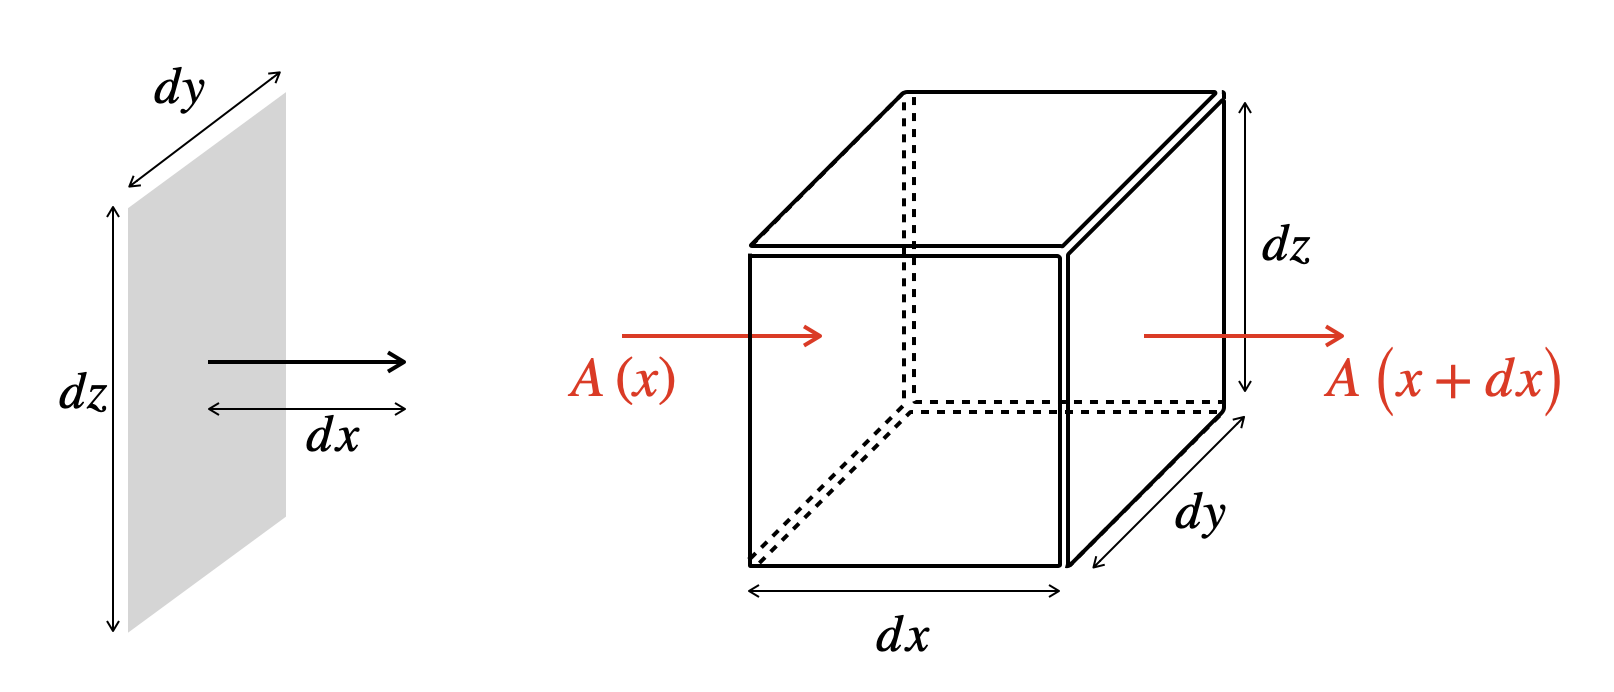
\includegraphics[scale=0.5]{figs/flux_any_diagram.png}
    \caption{$x$方向に空間を通過する$A$のイメージ}
    \label{flux_any_diagram}
\end{figure}


\section{力学}


\subsection{静水圧平衡}
静水圧平衡は、鉛直方向の気圧と重力の釣り合いを表す関係である。
\autoref{hydrostatic_diagram}のように微小格子を考え、重力と2格子間の気圧差 (気圧傾度力) が釣り合うとする。
このとき、ある格子に対して働く重力$G$は
\begin{equation}
    G = -\rho g dx dy dz
\end{equation}
一方、気圧傾度力$P$は
\begin{equation}
    P = \left(p\left(z\right) - p\left(z-dz\right)\right) dx dy = dp dx dy
\end{equation}
これらの議論から、静水圧平衡の式は次のように求まる
\begin{equation}
    \label{hydrostatic_balance}
    dp = -\rho g dz
\end{equation}
この式からわかる重要なことのひとつは、気圧は必ず高度が上がるごとに小さくなるということである。
つまり、気圧は単調減少し、逆転は起こらない。
この性質から、鉛直座標に気圧を用いた考察や計算がよく行われる。
\begin{figure}[t]
    \centering
    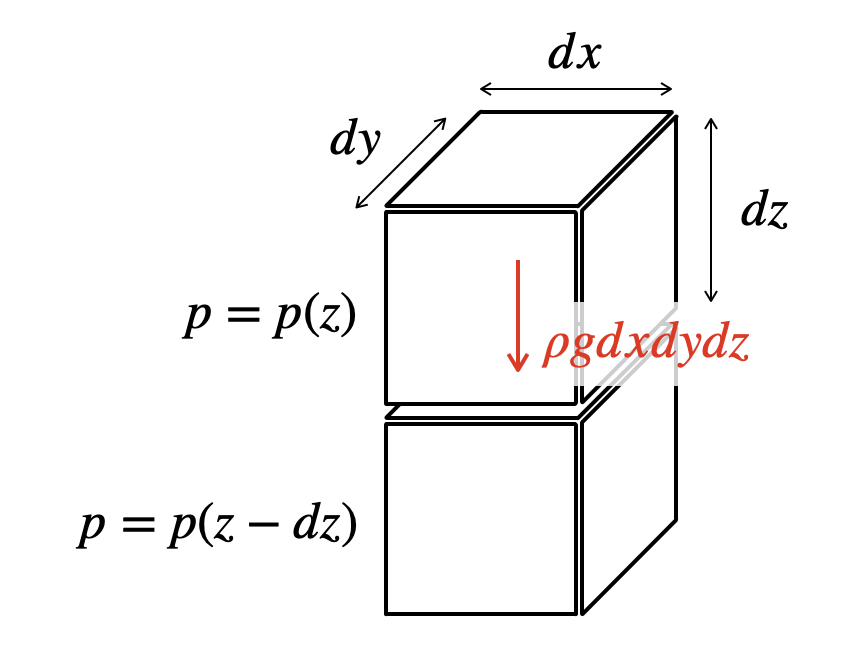
\includegraphics[scale=0.5]{figs/hydrostatic_diagram.png}
    \caption{静水圧平衡の模式図}
    \label{hydrostatic_diagram}
\end{figure}

静水圧平衡と状態方程式\autoref{equation_of_state}から、気圧と高度の関係を簡単に見積もってみる。
2つの式から$\rho$を消去することで
\begin{equation}
    dp = -{p \over RT} g dz
\end{equation}
温度を$T=273 \: \mathrm{K} = const.$として考えると、両辺の積分から
\begin{equation}
    p = p_0e^{-{z \over H}}
\end{equation}
ただし、地表気圧を$p_0$とし、$H=RT/g\sim 8 \:\mathrm{km}$を用いた。
すなわち、この条件では高度が$8 \:\mathrm{km}$高くなるごとに気圧が$1/e$になることがわかる。
このような高度をスケールハイトと呼び、大抵$H=7000 \: \mathrm{m}$か$H=8000 \: \mathrm{m}$が用いられる。
温度を一定とおく乱暴な近似に感じられるが、悪くない精度で高度と気圧の対応が得られることが知られている。


\subsection{運動方程式}
古典力学的には、質量を持った物体は運動方程式に従う。
大気を含む流体も質量を持って運動しているから、流体に対しても同様に運動方程式を定義できる。
ただし、流体の場合には単位体積あたりで考えるため、質量の代わりに密度$\rho$を使う。
流体に働く内力には、気圧傾度力、コリオリ力、摩擦力がある。
地球の自転による遠心力は万有引力と概ね並行な向きに働くため、万有引力との合力として重力を考え、顕に考えない。
以上をまとめると、流体の運動方程式はデカルト座標系で次のように表される
\begin{equation}
    \label{lagrange_eom}
    {d\vb*{v} \over dt} = -{1 \over \rho} \nabla p - \vb*{f} \cross \vb*{v} - \nabla \Phi + \vb*{X}
\end{equation}
ここで、$\vb*{v}$は風速、$p$は気圧、$\vb*{f}=2\vb*{\Omega}\sin{\phi}$はコリオリパラメータ、$\vb*{\Omega}$は地球の自転角速度ベクトル、$\phi$は緯度、$\Phi$はジオポテンシャル、$\vb*{X}$は摩擦力である。
ジオポテンシャル$\Phi$は重力ポテンシャルを表し、より正確には
\begin{equation}
    \Phi = \int^{z}_{0} dz \: gz
\end{equation}
で定義される。
これは地形や高度による重力加速度のムラを考慮した重力ポテンシャルの厳密な表現であるが、気象学で考える高度の範囲では重力加速度がほとんど一定であるため、大抵は$\Phi=gz$で考える。

さて、\autoref{lagrange_eom}は、ある空気の塊 (気塊, パーセル) の軌跡を追いかけながら運動を記述した表現である。
基本的な力学の文脈で質点速度の時間発展を考えたときと同じ表現と言える。
このような考えかたをラグランジュ法という。
しかし、流体力学では空間の速度分布に興味がある場合が多く、パーセルの速度がどのように変化したかには対しては興味が薄い。
すなわち、固定された座標に対して速度の時間発展を考える方が便利で、そのような考え方をオイラー法という。

ここからは、ラグランジュ的に考えた運動方程式をオイラー的な運動方程式に変換する。
微分のChain Ruleを考えればわかるように、任意物理量$A\left(t, x, y, z\right)$のラグランジュ的な時間微分は次のように書き換えることができる
\begin{equation}
    {dA \over dt} = \spartial{A}{t} + {dx \over dt}\spartial{A}{x} + {dy \over dt}\spartial{A}{y} + {dz \over dt}\spartial{A}{z}
\end{equation}
座標$\left(x, y, z\right)$の時間微分は速度$\left(u, v, w\right)$を表すから、この式は
\begin{equation}
    {dA \over dt}
    = \spartial{A}{t} + u\spartial{A}{x} + v\spartial{A}{y} + w\spartial{A}{z}
    = \spartial{A}{t} + \left(\vb*{v} \cdot \nabla\right)A
\end{equation}
最右辺の第1項は、ラグランジュ的な時間微分から座標変化による$A$の発展を取り除いた表現だから、ある固定座標における$A$の時間発展を表す。
すなわち、これはオイラー的な時間微分である。
第2項は移流項と呼ばれ、流速による$A$の輸送を表す。
これを使うと、オイラー法の運動方程式は
\begin{equation}
    \label{euler_eom}
    \spartial{\vb*{v}}{t} = -\left(\vb*{v} \cdot \nabla\right)\vb*{v} -{1 \over \rho} \nabla p - \vb*{f} \cross \vb*{v} - \nabla \Phi + \vb*{X}
\end{equation}
気象学では、よくこの表現を用いる。

以上では、デカルト座標系での運動方程式を紹介した。
一方で、気象学では鉛直座標に高度ではなく気圧を使うことも多い。
ここでは、鉛直座標を気圧として水平方向の成分のみを持ったベクトル演算子$\nabla_p$をもちいて、水平方向の運動方程式を考える。
重力加速度を定数とするから、\autoref{euler_eom}に現れた重力項をここでは考えない。
また、摩擦項も無視する。
静水圧平衡を用いると、$z$一定での水平微分と$p$一定での水平微分の関係は
\begin{equation}
    dA = \left(\spartial{A}{x}\right)_p dx + \left(\spartial{A}{p}\right)_x dp
\end{equation}
両辺を高度一定条件で$dx$で割ることで
\begin{equation}
    \label{A_z_p_conversion}
    \left(\spartial{A}{x}\right)_z = \left(\spartial{A}{x}\right)_p + \left(\spartial{A}{p}\right)_x \left(\spartial{p}{x}\right)_z
\end{equation}
よって、$A$に気圧$z$を代入することで、次が得られる
\begin{equation}
    0 = \left(\spartial{z}{x}\right)_p + \left(\spartial{z}{p}\right)_x \left(\spartial{p}{x}\right)_z
\end{equation}
最後に、\autoref{hydrostatic_balance}を用いれば
\begin{equation}
    \left(\spartial{p}{x}\right)_z = \rho g \left(\spartial{z}{x}\right)_p = \rho \left(\spartial{\Phi}{x}\right)_p
\end{equation}
よって、気圧傾度力は
\begin{equation}
    -{1 \over \rho}\left(\spartial{p}{x}\right)_z = -\left(\spartial{\Phi}{x}\right)_p
\end{equation}
この式を\autoref{euler_eom}に代入すれば、圧力座標での運動方程式が得られる
\begin{equation}
    \left(\spartial{\vb*{v}}{t}\right)_p = -u\left(\spartial{\vb*{v}}{x}\right)_p - v\left(\spartial{\vb*{v}}{y}\right)_p - \omega\spartial{\vb*{v}}{p} - \nabla_p \Phi- \vb*{f} \cross \vb*{v}
\end{equation}


\section{熱力学}


\subsection{温位}
高校物理で学ぶ熱力学第一法則から、非断熱加熱$Q$と内部エネルギー$U=c_vT$、仕事$pdV$の関係は次のように表される
\begin{equation}
    dQ = dU + p dV
\end{equation}
両辺を質量で割り、単位質量あたりの変化について考えると
\begin{equation}
    \label{thermal_first_law}
    dq = du + pd\alpha
\end{equation}
ただし$\alpha=1/\rho$。

大気のパーセルは、その運動を追跡すると非常によく断熱的に振る舞うことが知られている。
言い換えると、大気の熱拡散は移流に比べてあまり大きくなく、パーセル間の温度の交換はあまり大きくない。
このため、パーセルの運動について考えるとき、断熱を仮定することは有用である。
ここでは、\autoref{thermal_first_law}について断熱を仮定する。
単位質量あたりの定積比熱を$c_v$とおき、断熱仮定$dq=0$を考えると
\begin{equation}
    c_v dT = -pd\alpha = -d\left(p\alpha\right) + \alpha dp = -RdT + {dp \over \rho} = -RdT + {RT \over p}dp
\end{equation}
ただし、途中で\autoref{equation_of_state}を用いた。
単位質量あたりの定圧比熱$c_p$について$c_p=c_v+R$が成り立つから、この式は次のように書き換えられる
\begin{equation}
    {c_p \over R} {dT \over T} = {dp \over p}
\end{equation}
両辺の積分により、次のように温位と呼ばれる物理量$\theta$が定義される
\begin{equation}
    \theta = T \left({p_0 \over p}\right)^{R/c_p}
\end{equation}
ただし、$p_0$は地表気圧で、一般的に$p_0=1000 \: \mathrm{hPa}$が用いられる。
温位は、その導出過程からわかるように、パーセルを断熱的に地表へ移動させたときの温度を表す。
すなわち、高度間の気圧差による断熱圧縮/断熱膨張を考慮した潜在的な温度を意味し、鉛直方向の運動が重要となる現象では非常に重要となる物理量である。
また、大気の運動は、良く断熱的に振る舞うことからわかるように等温位面上を移動する。






\clearpage

\begin{thebibliography}{100}
    \item 北畠尚子, 2022 : 総観気象学 理論編, 気象庁, 285pp.
\end{thebibliography}

\end{document}

